%%%%%%%%%%%%%%%%%%%%%%%%%%%%%%%%%%%%%%%%%%%%%%%%%%%%%%%%%%%%%%%%%%%%%%%%%%%%%%%%
%2345678901234567890123456789012345678901234567890123456789012345678901234567890
%        1         2         3         4         5         6         7         8

%\documentclass[final,letterpaper, 10 pt, conference]{ieeeconf}  % Comment this line out if you need a4paper

%\documentclass[10pt, conference, compsocconf]{IEEEtran}
\documentclass[a4paper, 10pt, conference]{ieeeconf}      % Use this line for a4 paper

\IEEEoverridecommandlockouts                              % This command is only needed if
% you want to use the \thanks command

\newcommand{\eu}{\textrm{e}}
\newcommand{\figref}[1]{Fig.~\ref{fig:#1}}

\overrideIEEEmargins
\usepackage[obeyFinal]{todonotes}
\RequirePackage{graphicx}
\usepackage{subfigure}
\usepackage{bm}
%\usepackage{subequation}
\graphicspath{ {Figs/} }
\usepackage{url}
%\usepackage[tight,footnotesize]{subfigure}
\usepackage{fainekos-macros}


\usepackage{array}
\usepackage{url}


% See the \addtolength command later in the file to balance the column lengths
% on the last page of the document
\usepackage{amsmath} % assumes amsmath package installed
\usepackage{amssymb}  % assumes amsmath package installed
\renewcommand{\thefigure}{\arabic{figure}}
\title{\LARGE \bf Platform for Closed-Loop Testing of Implantable Cardiac Devices}

\author{ Marco Beccani, Kuk Jin Jang, Zhihao Jiang, Houssam Abbas and Rahul Mangharam% <-this % stops a space
	\thanks{*This work was supported by NSF Frontiers grant 1446664 and NSF CAREER grant 1253842}% <-this % stops a space
	\thanks{The Department of Electrical and Systems Engineering, University of Pennsylvania, Philadelphia, U.S.A.
		{\small
			 \{beccani,jangkj,zhihaoj,habbas,rahulm\}@seas.upenn.edu}}%
}

\begin{document}
	
\maketitle
\thispagestyle{empty}
\pagestyle{empty}

Implantable cardioverter–defibrillators (ICDs) are widely effective in reducing mortality rates by up to 31\% among patients affected by cardiac arrhythmias~\cite{Buxton1999}.  
ICDs stop a tachycardia (abnormally elevated heart rate) by delivering a high-energy electrical shock or a sequence of electrical pulses directly to the heart. 
This is known as \emph{therapy}.
Unfortunately, ICDs  suffer from a high rate of \emph{inappropriate therapy}: this is therapy delivered to non-fatal SupraVentricular Tachycardias (SVT), rather than to fatal Ventricular Tachycardias (VT).
Depending on the particular ICD and its settings, inappropriate therapy rates range from 46\% to 62\% of all delivered therapy, increasing patient stress and reducing the quality of their life \cite{shock_mortality}. 
ICD safety and efficacy is therefore a serious problem that has to be addressed.

\begin{figure}[h]
	\centering
	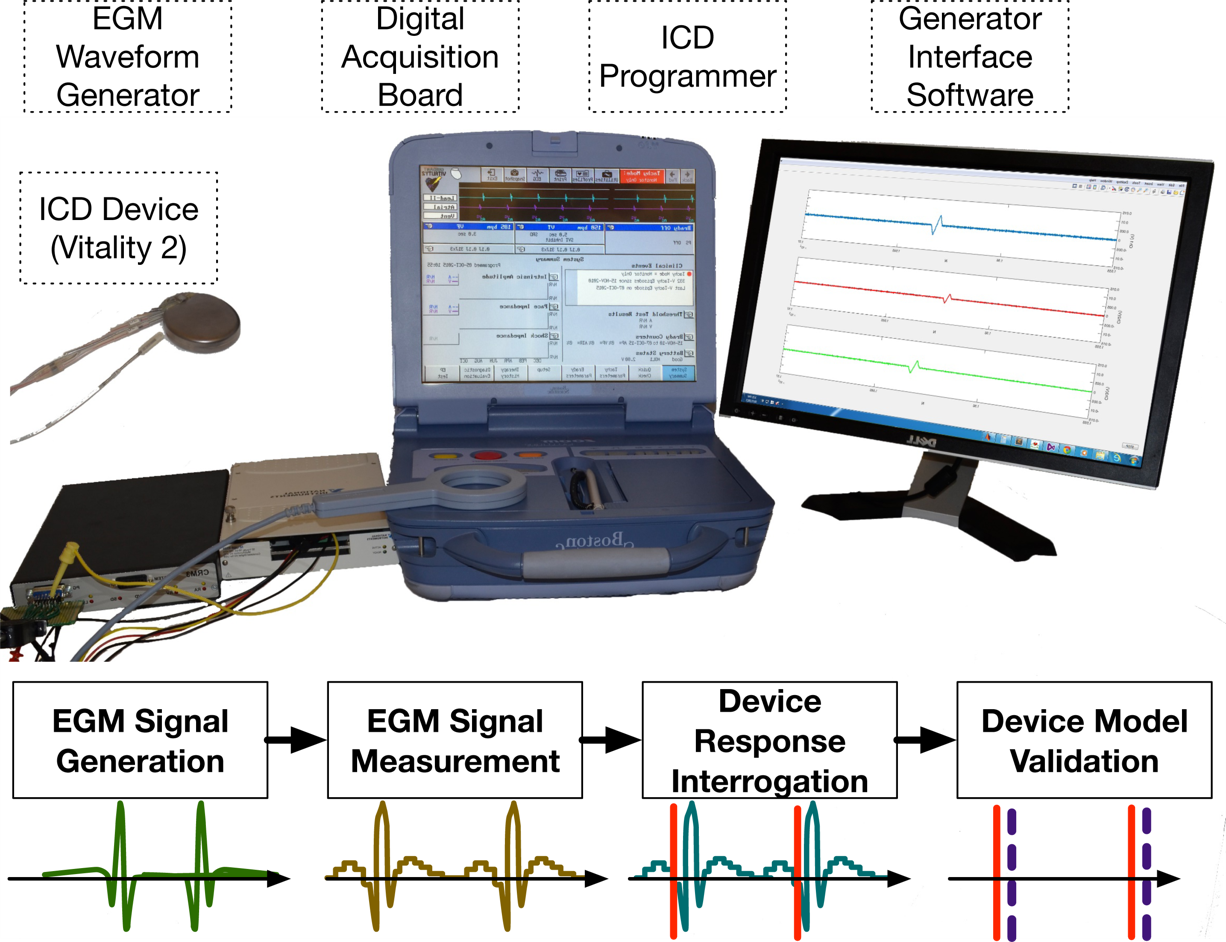
\includegraphics[scale=0.32]{Fig1.png}
	\caption{\small Experimental setup. The programmer is used to trace the decision process of the ICD as it determines whether to deliver therapy.}
	\vspace{-10pt}
	\label{fig:1}
\end{figure}

We present a platform that can be used for testing the closed-loop safety and efficacy of an ICD. 
Computer models of the heart are used to generate heart signals reproducing different tachycardias.
Synthetic heart signals are then fed into a real ICD device.
This allows designers to understand the conditions that are more likely to cause inappropriate therapy, and it allows other parties like regulators and potential customers to assess the safety and efficacy of an ICD.

Our experimental setup is represented in Fig.~\ref{fig:1}.
It consists of a PC running the signal generation software, a National Instruments Data Acquisition (DAQ), and an ICD  (Vitality II from Boston Scientific). 
We simulated 8 different tachycardias, reproducing real patient signals, as listed in details in Table \ref{tab:1}.  
Heart signals are generated by the DAQ board and are then fed into the ICD sensing leads. 
These are the leads that are normally implanted in the heart muscle.
Furthermore an ICD programmer (ZOOM Latitiude from Boston Scientic) was used to verify if the shock occurred.

\begin{figure}[t]
	\centering
	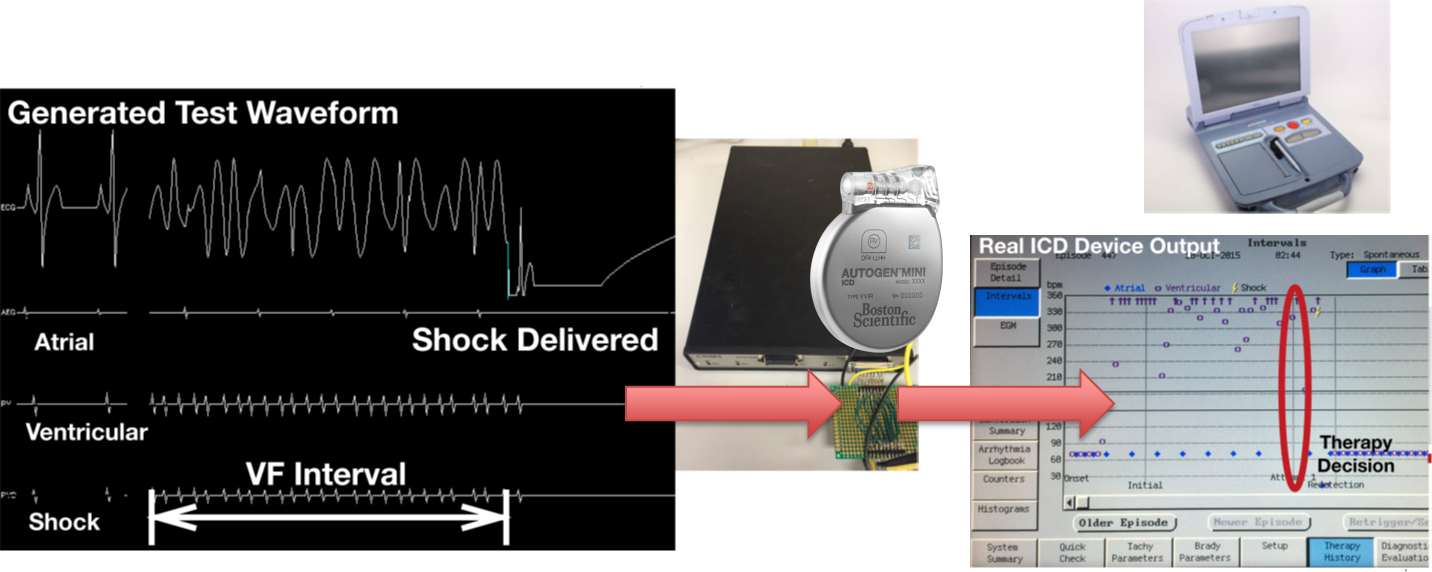
\includegraphics[scale=0.32]{Fig2.png}
	\caption{\small The platform output screenshots during VF  (Ventricular brillation) showing the therapy delivery decision for the ICD.}
	\vspace{-5pt}
	\label{fig:2}
\end{figure}

Fig.~\ref{fig:2} illustrates one such tachycardia scenario, specifically Ventricular Fibrillation (VF). In this case, the actual ICD  therapy was delivered as a consequence of the generated VF waveform.

\begin{table}
\caption{Sample results of tested tachycardias}
\begin{tabular}{|p{2in}|p{1in}|}
	\hline \textbf{Arrhythmia} & \textbf{Therapy Deliver} \\
	\hline Atrial Fibrillation & No\\
	\hline Atrial Flutter & No\\
	\hline Premature ventricular complexes & No \\
	\hline Nonsustained ventricular tachycardia & No\\
	\hline Other Supraventricular tachycardia & No \\
	\hline Brady-Tachy & No \\
	\hline Ventricular fibrillation & Yes \\
	\hline Ventricular tachycardia & Yes \\
	\hline
\end{tabular}
\vspace{-10pt}
\label{tab:1}
\end{table}


The platform hereby presented has the potential in the future to enable new methodologies of verification and testing for commercial ICDs.  
Therefore it contributes to the ongoing evolution of ICD therapy for primary prevention aiming to reduce potentially dangerous inappropriate therapies and increased survival among patients with ICDs.


	\bibliographystyle{IEEEtran}%abbrv}
	\bibliography{IEEEabrv,bibliography}
	
\end{document}

